\documentclass[multi=false,tikz,border=2mm]{standalone}
\usetikzlibrary{arrows,decorations.markings}

\usepackage{tikz}
\begin{document}
\tikzset{triangle/.pic={
		code={
			\draw[very thick] (-2,-3) -- (2,-3) -- (0, 0) -- cycle;
		}
	}
}
\tikzset{revtriangle/.pic={
		code={
			\draw[very thick] (2,3) -- (-2,3) -- (0, 0) -- cycle;
		}
	}
}

\begin{tikzpicture}
	\draw [very thick] (0,3) -- (0,-5);
	\path (0,0) pic {revtriangle};
\end{tikzpicture}
\begin{tikzpicture}
	\draw [very thick] (0,0) -- (0,1);
	\path (0,0) pic {triangle};
	\path (0,1) pic {revtriangle};
\end{tikzpicture}

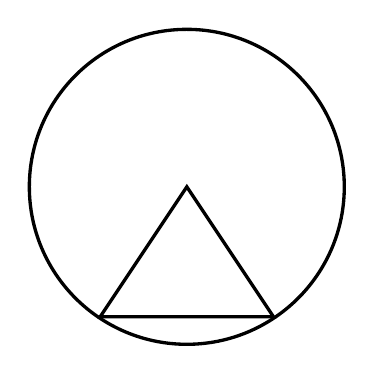
\begin{tikzpicture}
	\draw[very thick] (0,0) circle (2cm);
	\draw[very thick] (-1.1,-1.65) -- (0,0) -- (1.1,-1.65) -- cycle;
\end{tikzpicture}

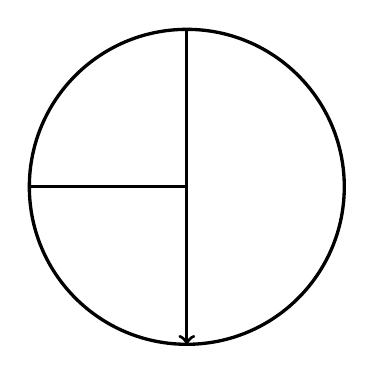
\begin{tikzpicture}
	\draw[very thick] (0,0) circle (2cm);
	\draw[->,very thick] (-2,0) -- (0,0) -- (0,-2);
	\draw[very thick] (0,0) -- (0,2);
\end{tikzpicture}
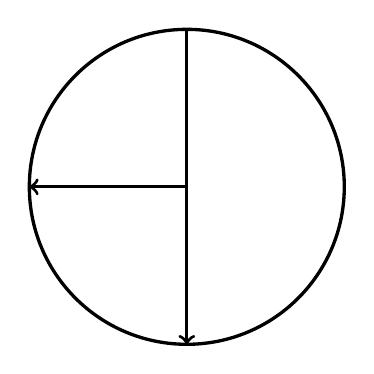
\begin{tikzpicture}
	\draw[very thick] (0,0) circle (2cm);
	\draw[->,very thick] (0,0) -- (-2,0);
	\draw[->,very thick] (0,0) -- (0,-2);
	\draw[very thick] (0,0) -- (0,2);
\end{tikzpicture}
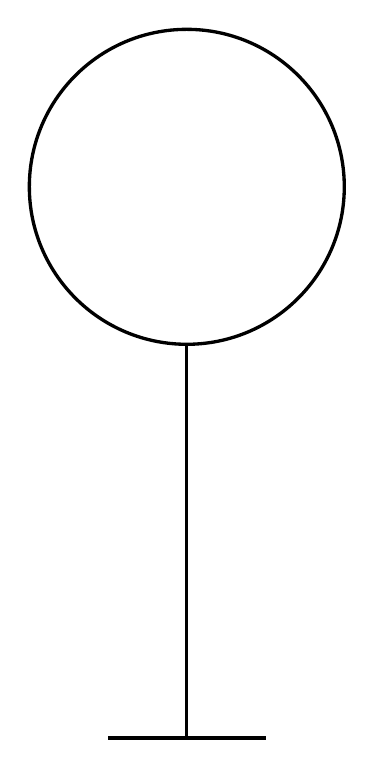
\begin{tikzpicture}
	\draw[very thick] (0,0) circle (2cm);
	\draw[very thick] (0,-2) -- (0,-7);
	\draw[very thick] (-1,-7) -- (1,-7);


\end{tikzpicture}
\begin{tikzpicture}
	\path (0,0) pic {triangle};

\end{tikzpicture}

\end{document}
